\chapter{Doświadczenia praktyczne z pracy z systemem}
\label{chap:Testy}

 

 W~ramach tej pracy wykonano prototypową instalację i~konfigurację
 rozbudowanego systemu {\em Icinga}, która została uruchomiona
 w~niewielkiej sieci domowej. W ramach instalacji uruchomiono również
 opracowany dodatek NSCAv2, do którego z powodzeniem podłaczono dwa
 urządzenia mobilne pod kontrolą aplikacji monitorującej IcingaMini
 \cite{book:pracaKubika}. Pozwoliło to na uruchomienie kompletnego
 systemu oraz weryfikację poprawności jego implementacji
 i~zdefiniowanych wymagań.

\section[Opis infrastruktury][Opis infrastruktury]{Opis infrastruktury}

Konfiguracja systemu Icinga (wraz z~szeregiem dodatków) została
wykonana w~mieszkaniu autora pracy w~oparciu o~istniejącą
infrastrukturę sieci lokalnej. Sercem konfiguracji jest laptop HP
Compaq 6710b. Został na nim zainstalowany system operacyjny
Linux. Wybrano najnowszą dostępną w~czasie wykonywania konfiguracji,
wersję dystrybucji Ubuntu --- 13.10. System został zainstalowany
w~wersji 64-bitowej. W~celu zapewnienia możliwości łatwego
przeniesienia wykonanej konfiguracji systemu monitorującego, utworzono
na tym serwerze maszynę wirtualną. Do jej stworzenia użyto narzędzi
opartych o~bibliotekę {\em libvirt}. Maszyna wirtualna uruchamiana
jest jako KVM\footnote{ang. {\em Kernel Virtual Machine} -- sposób
  wirtualizacji w~systemach Linuksa, gdzie proces ten jest wspierany
  przez jądro systemu gospodarza}, co zapewnia jej wysoką
wydajność. Na utworzonej maszynie wirtualnej zainstalowany został ten
sam system operacyjny, co na urządzeniu będącym jej
gospodarzem. Interfejs sieciowy urządzenia został skonfigurowany
w~taki sposób, aby urządzenie fizyczne i~maszyna wirtualna widziane
były z~zewnątrz jako dwa interfejsy o~różnych adresach MAC.

Poza laptopem oraz maszyną wirtualną w~sieci dostępne są również inne
urządzenia. Pierwszym z~tych urządzeń jest drukarka sieciowa Samsung
CLP-610ND. Posiada ona interfejs sieciowy, na którym udostępniana jest
usługa bezpośredniego drukowania i~administracji poprzez stronę
internetową z~użyciem protokołu HTTP. Drugie urządzenie to router ASUS
WL-500GPv2. Jest to element odpowiedzialny za przydział adresów
w~całej sieci z~użyciem protokołu DHCP. Ponadto jest on bramą domyślną
dla wszystkich urządzeń znajdujących się w~sieci lokalnej. Wyposażony
jest w~interfejs zarówno przewodowy, jak i~bezprzewodowy. Urządzenie
to udostępnia panel administracyjny w~formie strony internetowej
poprzez protokół HTTP. Ponadto w~sieci znajduje się przełącznik ASUS
GigaX 1005/G, dzięki któremu urządzenia połączone są w~sieć lokalną
bez konieczności korzystania z~routera. W~dalszych rozważaniach
urządzenie to zostało pominięte, ponieważ jest to prosty przełącznik
warstwy drugiej i~nie jest możliwe jego monitorowanie.

Testowa sieć lokalna zawiera zdecydowanie zbyt mało elementów, aby móc
w~pełni przetestować działanie systemu. Ponadto jest ona w~znacznym
stopniu odizolowana od czynników zewnętrznych mogących wpływać na
pracę systemu monitorującego. W~celu wykonania bardziej realistycznych
testów postanowiono monitorować dwa dostępne publicznie
serwery. Pierwszym z~nich jest serwer {\em google.com}. Drugi
natomiast to serwer {\em mion.elka.pw.edu.pl} przeznaczony dla
studentów Wydziału Elektroniki i~Technik Informacyjnych Politechniki
Warszawskiej.

W~ramach niniejszej pracy wykonano rozbudowę systemu monitorującego
{\em Icinga} o~funkcjonalność monitorowania klienta
mobilnego. W~związku z~powyższym konieczne było uwzględnienie również
klientów mobilnych w~konfiguracji testowej. Dzięki uprzejmości Pana
Marcina Kubika możliwe było wykorzystanie opracowanego przez niego
modułu mobilnego dla platformy Android (smartfon Samsung Galaxy Note 3
oraz Samsung Galaxy S2 Plus). Pozwoliło to na dodanie do monitorowanej
infrastruktury dwóch urządzeń mobilnych pracujących pod kontrolą tego
systemu. Oba urządzenia były używane do codziennych czynności, co
pozwoliło na symulacje normalnych warunków pracy systemu.

Aby umożliwić komunikację aplikacji mobilnej z~dodatkiem NSCAv2 spoza
sieci domowej, konieczne było użycie mechanizmu przekazywania portów
na wspomnianym wcześniej routerze. Schemat wykonanej testowej
infrastruktury przedstawiono na rysunku \ref{fig:schematSieci}. Na
schemacie zachowano porządek oznaczeń urządzeń przedstawiony w~tabeli
\ref{tab:devices}.

\begin{figure}[ht]
  \caption{Schemat infrastruktury testowej. Kolorem czerwonym zostało
    wyróżnione połączenie wynikające z~przekierowania portów.}
  \label{fig:schematSieci}
  \centering
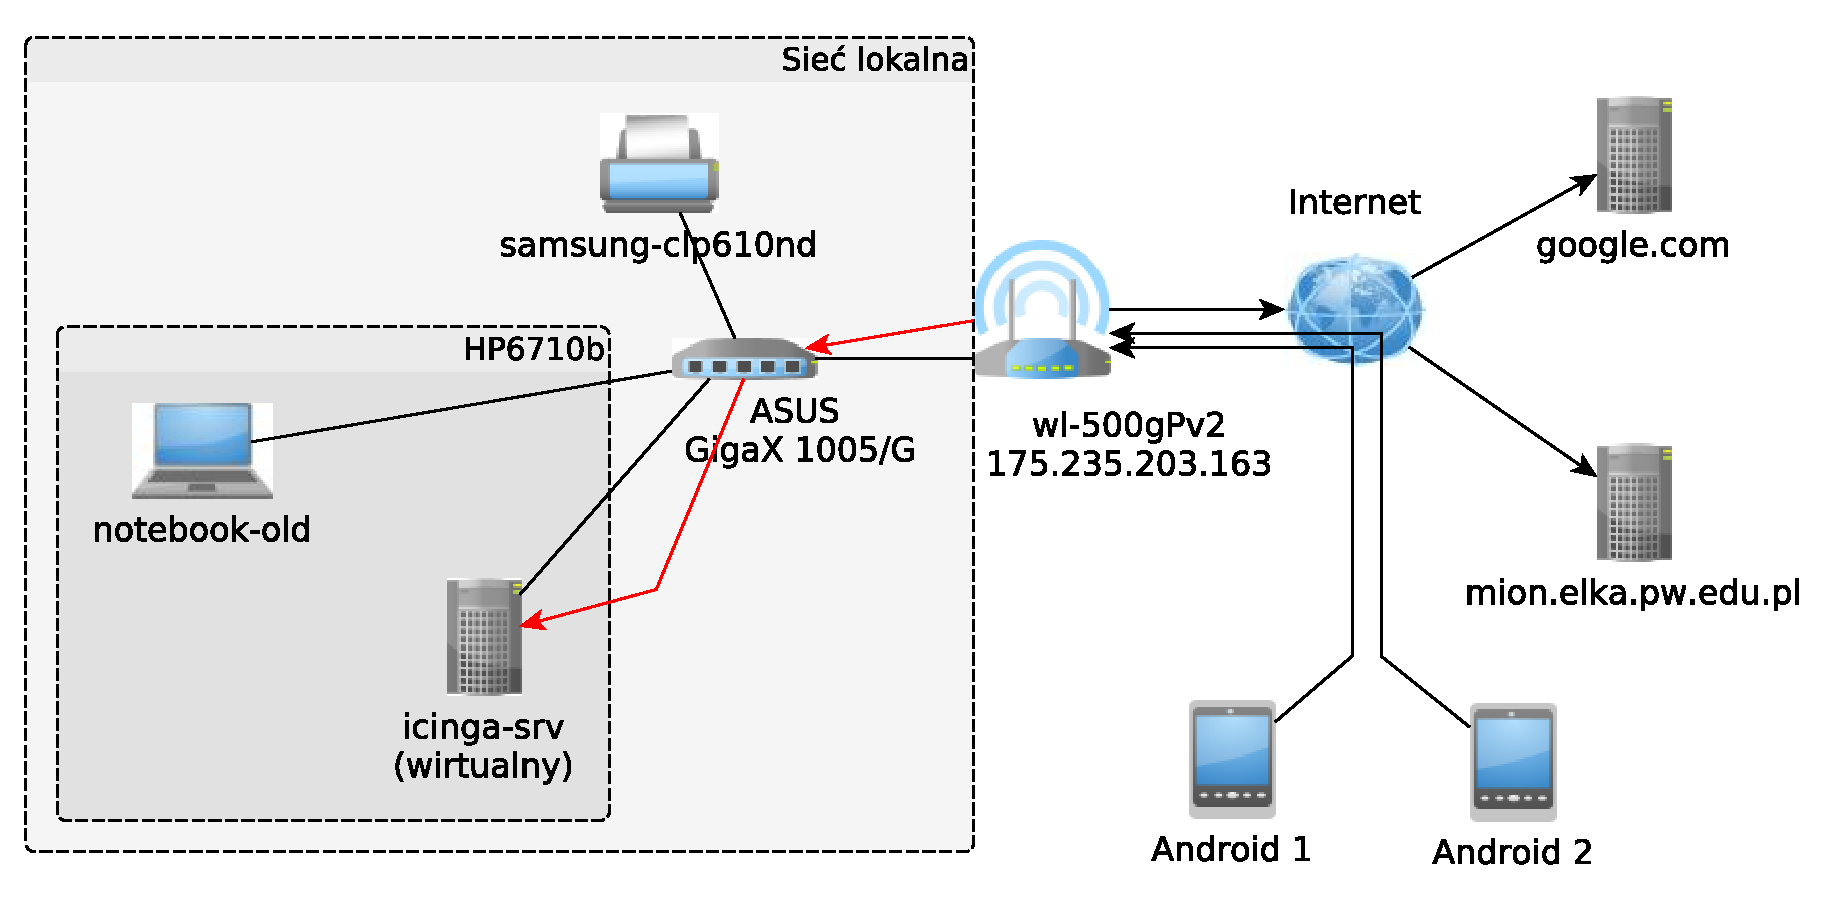
\includegraphics[width=1\textwidth]{img/schematSieci}
\end{figure}

\begin{table}
\centering
\caption{Objaśnienia nazw urządzeń wykorzystywanych w~infrastrukturze.}
\label{tab:devices}
\begin{tabular}{|p{4cm}||p{10cm}|}
  \hline
  Nazwa & Opis \\
  \hline \hline
  notebook-old & System zainstalowany natywnie na laptopie HP 6710b. \\
  \hline
  icinga-srv & System uruchomiony na maszynie wirtualnej na urządzeniu notebook-old. \\
  \hline
  samsung-clp610nd & Drukarka Samsung CLP-610ND znajdująca się w sieci lokalnej \\
  \hline
  \raggedright{wl-500gPv2 175.235.203.163} & \raggedright{Router ASUS WL-500GPv2 o zewnętrznym adresie IP 175.235.203.163}
  \tabularnewline
  \hline
  google.com & Serwer popularnej wyszukiwarki internetowej Google. \\
  \hline
  mion.elka.pw.edu.pl & Serwer mion zarządzany przez WEiTI PW. \\
  \hline
  Android 1 & Telefon Samsung Galaxy Note 3. \\
  \hline
  Android 2 & Telefon Samsung Galaxy S2 Plus. \\
  \hline
\end{tabular}
\end{table}

\section[Konfiguracja systemu monitorowania][Konfiguracja systemu
monitorowania]{Konfiguracja systemu monitorowania}

Monitorowana infrastruktura jest dość prosta i~mała. Pozwala to na
użycie jednego rdzenia monitorującego zarówno do monitorowania
infrastruktury statycznej, jak i~do przetwarzania danych pochodzących
od klientów mobilnych. W~celu zapewnienia konfiguracji zbliżonej do
warunków użytkowania systemu, wykonano konifgurację wraz z dodatkien
inGraph oraz bazą danych dla systemu {\em Icinga}. Konfiguracja całego
systemu składa się z~następujących elementów:

\begin{itemize}
\item rdzeń monitorujący {\em Icinga},
\item baza danych MySQL systemu {\em Icinga},
\item dodatek inGraph,
\item baza danych MySQL dodatku inGraph,
\item interfejs icinga-web,
\item baza danych MySQL icinga-web\footnote{Ze względu na użycie
    nowego interfejsu konieczna jest dodatkowa baza danych, w~której
    przechowywane są dane warstwy prezentacji. Baza ta nie została
    wymieniona w~opisie, gdyż nie zawiera ona danych o stanie sieci,
    a~jedynie dane interfejsu graficznego.},
\item wykonany w~tej pracy dodatek NSCAv2,
\item aplikacja mobilna dla platformy Android, napisana przez Pana
  Kubika,
\item zestaw wtyczek.
\end{itemize}

Schemat rozmieszczenia oraz współpracy poszczególnych elementów został
przedstawiony na rysunku~\ref{fig:deployment}. System monitorowania do
poprawnego funkcjonowania potrzebuje zarówno serwera bazy danych
MySQL, jak i~serwera http. W~wykorzystywanej wersji dystrybucji Ubuntu
wymagane pakiety zostały zainstalowane domyślnie podczas instalacji
systemu.

\begin{figure}[ht]
  \caption{Diagram rozmieszczenia i~współpracy elementów systemu
    monitorowania.}
 \label{fig:deployment}
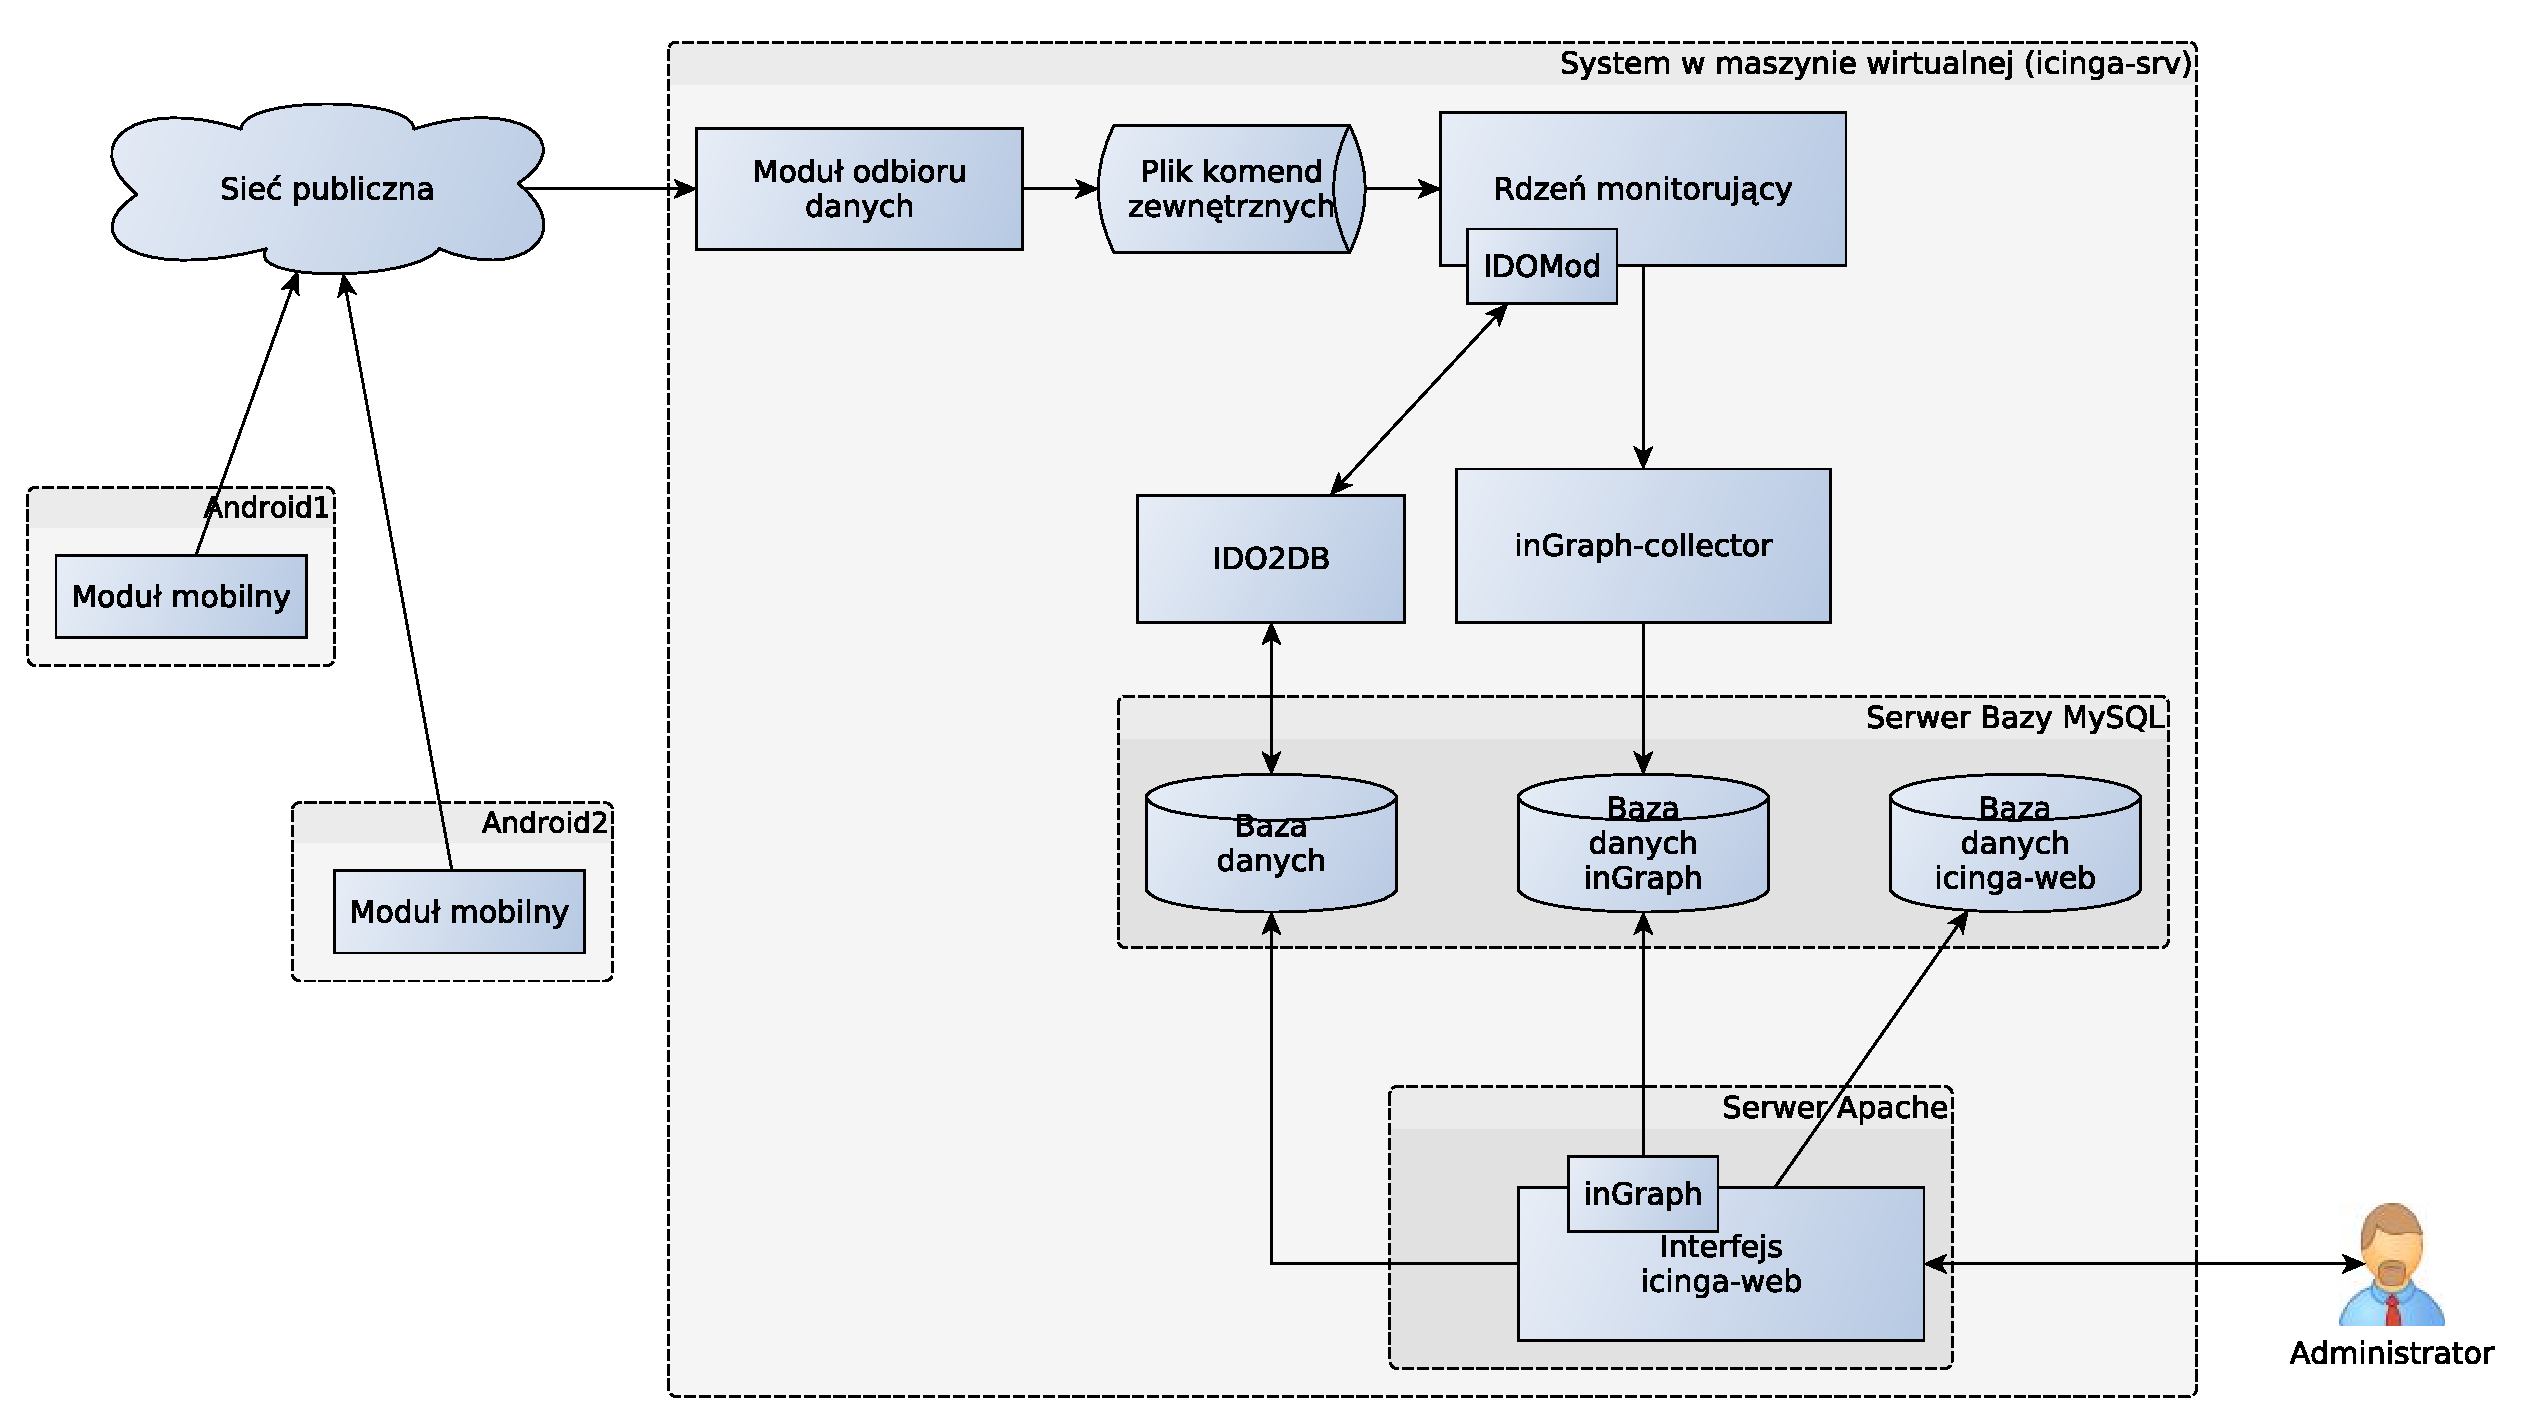
\includegraphics[width=1\textwidth]{img/deployment}
\end{figure}

Rdzeń systemu monitorowania został skonfigurowany tak, aby monitorować
w~sposób aktywny wszystkie usługi klientów statycznych. Do
monitorowania użyto zestawu standardowych wtyczek rozwijanych
pierwotnie dla systemu Nagios. Lista monitorowanych usług dla każdego
urządzenia została przedstawiona w~formie tabeli
\ref{tab:hostServiceStatic}. Niektóre z~monitorowanych wartości
wymagają użycia dodatkowego narzędzi - NRPE\footnote{ang. {\em Nagios
    Remote Plugin Executor} -- narzędzie do zdalnego uruchamiania
  wtyczek. Dokładny opis można znaleźć w~\cite{www:NRPE}.}. Jest to
narzędzie, które pozwala na uruchomienie wtyczki na zdalnej
maszynie. Jest on niezbędny do pomiaru parametrów wewnętrznych danego
urządzenia, takich jak zużycie procesora czy pamięci. Użyto go do
minitorowania systemu gospodarza (laptop).

\begin{table}
\centering
\caption{Monitorowane usługi i parametry klientów statycznych}
\label{tab:hostServiceStatic}
\begin{tabular}{|p{2.5cm}|c|p{2cm}|p{2cm}|c|c|c|}
\hline
\raggedright{Wartość mierzona} & icinga-srv & \raggedright{notebook- -old} & \raggedright{samsung- -clp610nd} & wl-500gPv2 & google & mion \\
\hline
\raggedright{Liczba procesów} & \multicolumn{1}{|c|}{Tak} & \multicolumn{1}{|c|}{Tak}  &   &  &  &  \\
\hline

\raggedright{Użycie przestrzeni wymiany} & \multicolumn{1}{|c|}{Tak} &  &  &  &  &  \\
\hline

SSH & \multicolumn{1}{|c|}{Tak} & \multicolumn{1}{|c|}{Tak} &  &  &  & \multicolumn{1}{|c|}{Tak} \\
\hline

Użycie dysku & \multicolumn{1}{|c|}{Tak} &  &  &  &  &  \\
\hline

HTTP & \multicolumn{1}{|c|}{Tak} & \multicolumn{1}{|c|}{Tak} & \multicolumn{1}{|c|}{Tak} & \multicolumn{1}{|c|}{Tak} & \multicolumn{1}{|c|}{Tak} & \multicolumn{1}{|c|}{Tak} \\
\hline

\raggedright{Liczba zalogowanych użytkowników} & \multicolumn{1}{|c|}{Tak} & \multicolumn{1}{|c|}{Tak} &  &  &  &  \\
\hline

\raggedright{Bieżące obciążenie} & \multicolumn{1}{|c|}{Tak} & \multicolumn{1}{|c|}{Tak} &  &  &  &  \\
\hline

Ping & \multicolumn{1}{|c|}{Tak} & \multicolumn{1}{|c|}{Tak} & \multicolumn{1}{|c|}{Tak} & \multicolumn{1}{|c|}{Tak} & \multicolumn{1}{|c|}{Tak} & \multicolumn{1}{|c|}{Tak} \\
\hline

\raggedright{Liczba procesów} & \multicolumn{1}{|c|}{Tak} &  &  &  &  &  \\
\hline

IMAP z SSL &  &  &  &  &  & \multicolumn{1}{|c|}{Tak} \\
\hline

POP3 z SSL &  &  &  &  &  & \multicolumn{1}{|c|}{Tak} \\
\hline

SMTP &  &  &  &  &  & \multicolumn{1}{|c|}{Tak} \\
\hline

\raggedright{Liczba procesów zombie} &  & \multicolumn{1}{|c|}{Tak} &  &  &  &  \\
\hline
\end{tabular}
\end{table} 

W celu umożliwienia monitorowania klienta mobilnego konieczne było
również zdefiniowanie w~systemie {\em Icinga} urządzeń Android1 oraz
Android2, a~także odpowiednich usług. Udostępniona przez Pana Marcina
Kubika wersja aplikacji mobilnej posiada duży zbiór parametrów
urządzenia, które można monitorować. Spośród dostępnych parametrów
wybrano następujące:

\begin{itemize}
\item siła najmocniejszego sygnału Wi-Fi,
\item stan baterii,
\item liczba uruchomionych aplikacji,
\item obciążenie procesora.
\end{itemize}

Konieczna była również konfiguracja dodatku NSCAv2. Ponieważ telefony
posiadały różnych użytkowników, zostały utworzone dwa konta
klientów. Jako jedyną dopuszczalną metodę uwierzytelnienia wybrano
login oraz hasło. W~celu zapewnienia transportu danych konieczne było
również nadanie utworzonym użytkownikom uprawnień dotyczących urządzeń
i usług. W~celu umożliwienia przesłania danych od klienta konieczna
była konfiguracja dostawcy danych. Pierwszym jej etapem było
wygenerowanie pary kluczy RSA oraz umieszczenie klucza prywatnego
i~publicznego na serwerze, a~publicznego na urządzeniach
mobilnych. Konieczne było również podanie w~pliku konfiguracyjnym
dodatku NSCAv2 ścieżki do klucza prywatnego, a~także numeru portu na
którym powinien on czekać na przychodzące połączenia. Ponieważ plik
komend zewnętrznych w~wykonanej instalacji systemu {\em Icinga} znajduje się
w~standardowym miejscu, konieczna była jedynie bezparametrowa
deklaracja konsumenta danych. Ostatnim etapem konfiguracji było
zdefiniowanie ścieżki danych dla klientów, prowadzącej od dostawcy
danych do odbiorcy.

Przedstawiona na rys.~\ref{fig:schematSieci} topologia sieci wyraźnie
pokazuje, że istnieje w~sieci urządzenie, którego awaria może
spowodować utratę łączności z~wieloma urządzeniami. Elementem tym jest
router wl-500gpv2. Awaria tego urządzenia powoduje, że serwer icinga
traci możliwość wykonywania sprawdzeń zarówno tego urządzenia, jak
i~wszystkich urządzeń znajdujących się poza siecią lokalną. W~celu
ograniczenia liczby komunikatów otrzymywanych w~przypadku takiej
awarii konieczne było zdefiniowanie odpowiedniej struktury
sieci. Rysunek \ref{fig:logicznySchematSieci} przedstawia logiczną
strukturę połączeń. Została ona wygenerowane przez program {\em Icinga} na
podstawie plików konfiguracyjnych monitorowanych urządzeń. Łatwo
zauważyć, że jedyna ścieżka od systemu monitorującego do wszystkich
urządzeń spoza sieci lokalnej prowadzi przez router
wl-500gpv2. Odpowiada to oczywiście fizycznym zależnościom w~sieci
i~umożliwi precyzyjną diagnozę ewentualnej awarii.

\begin{figure}[ht]
  \caption{Logiczny schemat monitorowanej
    infrastruktury.}
  \label{fig:logicznySchematSieci}
  \centering
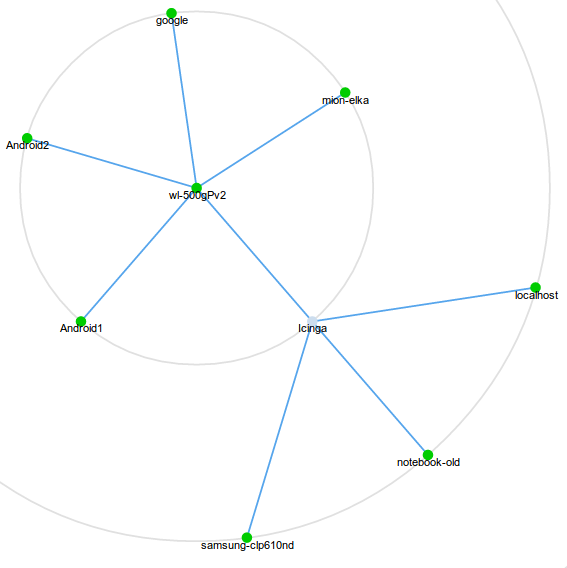
\includegraphics[width=0.8\textwidth]{img/logicznySchematSieci.png}
\end{figure}

\section[Klient statyczny][Rezultaty dla klientów statycznych]{Rezultaty dla klientów statycznych}

Monitorowanie infrastruktury statycznej zostało przeprowadzone
w~okresie trzech tygodni. Czas ten jest zdecydowanie wystarczający, aby
zgromadzić dane, będące wiarygodnym źródłem informacji o~sieci. Należy
zauważyć, że system monitorowania działał przez cały ten czas bez
żadnej awarii.

\subsection[Sieć lokalna][Sieć lokalna]{Sieć lokalna}

Testowanie monitorowania sieci lokalnej przebiegło zgodnie
z~oczekiwaniami. Zgromadzone dane wykazały stałą jakość usług
świadczonych w~sieci lokalnej. Ze względu na niski poziom
skomplikowania infrastruktury testowej, otrzymywane wartości czasu od
wysłania pakietu do jego powrotu były rzędu pojedynczych
milisekund. Dzięki wykorzystaniu dodatku inGraph możliwe było
przedstawienie zgromadzonych danych w~formie wykresów.

Przykładowy wykres czasu podróży pakietów oraz poziomu utraconych
podczas komunikacji pakietów dla router wl-500gPv2 przedstawiono na
rys.~\ref{fig:pingRoutera}. Na wykresie kolorem zielonym zostały
zaznaczone średnie czasy podróży dla zadanych przedziałów. Kolor szary
prezentuje natomiast wartości minimalne i~maksymalne dla bieżących
przedziałów agregacji. Kolor czerwony pokazuje udział utraconych
pakietów wobec wszystkich przesłanych.

\begin{figure}[ht]
  \caption{Wykres wartości czasu podróży pakietu oraz stopnia
    utraconych pakietów dla wl-500gPv2. Wykresy przedstawiają
    odpowiednio okres jednego dnia, tygodnia oraz miesiąca.}
  \label{fig:pingRoutera}
  \centering
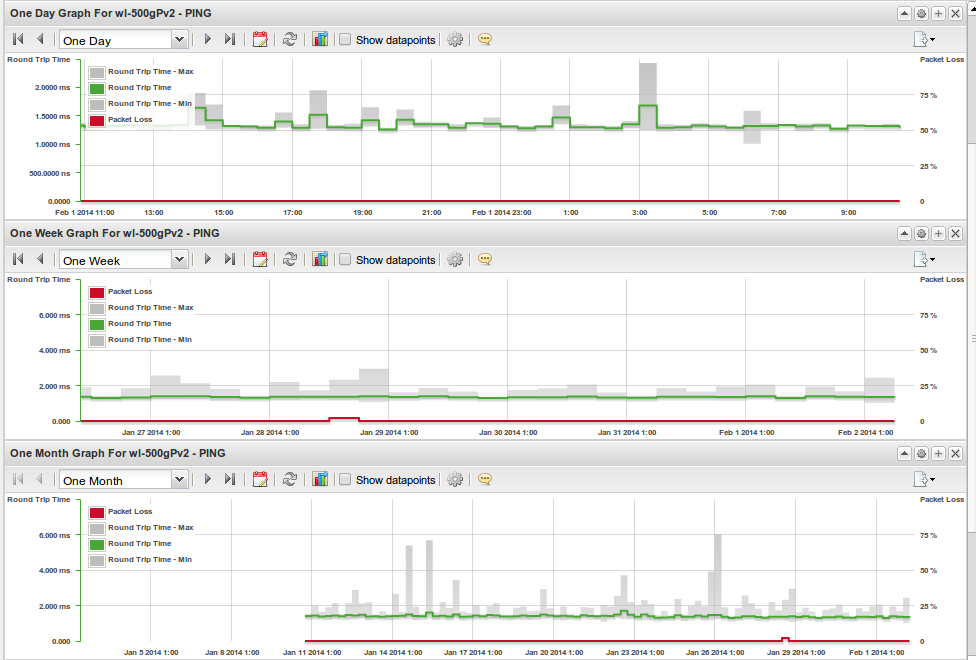
\includegraphics[width=1\textwidth]{img/pingRoutera.png}
\end{figure}

Przedstawiony wykres potwierdza prawidłowe wyniki przeprowadzonych
testów systemu. Średni czas podróży pakietu wynosi poniżej 2
ms. Uzyskane wartości maksymalne są rzędu 6 ms, co również jest
zjawiskiem normalnym w~sieciach komputerowych, ze względu na zmienne
obciążenie routera. Należy zauważyć, że na wykresie wystąpił chwilowy
wzrost stopnia utraconych pakietów w~okolicach 29 stycznia. Dodatek
inGraph pozwala administratorowi, po zauważeniu takiej sytuacji
wygenerować wykres dokładniejszych wartości we wskazanym
okresie. Funkcja szybkiego widoku, która pozwala na zaznaczenie
interesującego obszaru pozwoliła na łatwe przedstawienie dokładnych
danych z~okresu wystąpienia wzrostu mierzonej wartości. Wykres ten
został przedstawiony na rysunku \ref{fig:pingRouteraDokladny}. Na
podstawie tego wykresu można określić dokładny czas wystąpienia
interesującego zdarzenia. W~przypadku wystąpienia usterki może to
zostać wykorzystane do diagnozowania jej przyczyny poprzez badanie
zdarzeń tuż przed jej wystąpieniem.

\begin{figure}[ht]
  \caption{Wykres wartości czasu podróży pakietu oraz stopnia
    utraconych pakietów dla wl-500gPv2 w okresie, gdzie wystąpił
    wzrost stopnia utraconych pakietów.}
  \label{fig:pingRouteraDokladny}
  \centering
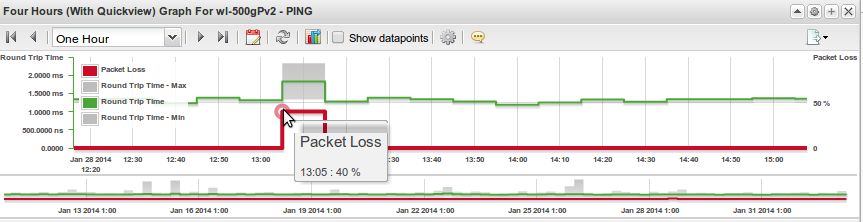
\includegraphics[width=1\textwidth]{img/pingiRouterDokladny.png}
\end{figure}

\subsection[Serwery zewnętrzne][Serwery zewnętrzne]{Serwery zewnętrzne}

Sieć lokalna jest wykorzystywana jedynie przez wąskie grono
użytkowników. Powoduje to niewielką zmienność monitorowanych w~niej
parametrów. Dzięki monitorowaniu serwerów zewnętrznych możliwe było
przetestowanie systemu w~dużo bardziej realistycznych warunkach.

Monitorowanie popularnego i~ogólnodostępnego serwera {\em google.com}
pozwoliło na przetestowanie systemu z~realnym systemem o~dużym
i~bardzo zmiennym obciążeniu. Rezultaty monitorowania serwisu zostały
przedstawione w~formie wykresu na rys.~\ref{fig:pingiGoogle}. Nawet
pobieżna analiza takiego wykresu pozwala zauważyć obecne w~nim
trendy. Na podstawie wykresu miesięcznego można zauważyć cykliczne
wzrosty wartości maksymalnej dla zadanych przedziałów
agregacji. Wykres ten pokazuje, iż występują one praktycznie
codziennie. Analiza wykresu tygodniowego pozwala dodatkowo na
określenie, że wspomniane skoki wartości maksymalnej występują
w~godzinach wieczornych. Ponadto łatwo zauważyć, że każdego dnia
w~godzinach popołudniowych i~wieczornych występuje znaczny wzrost
średniego czasu odpowiedzi serwera. Dzięki dynamicznemu charakterowi
wykresów programu inGraph możliwe jest dokonanie dokładnej analizy
widocznych na wykresie tendencji.

\begin{figure}[ht]
  \caption{Wykres wartości czasu podróży pakietu oraz stopnia
    utraconych pakietów dla google.com.  Wykresy przedstawiają
    odpowiednio okres jednego dnia, tygodnia oraz miesiąca.}
  \label{fig:pingiGoogle}
  \centering
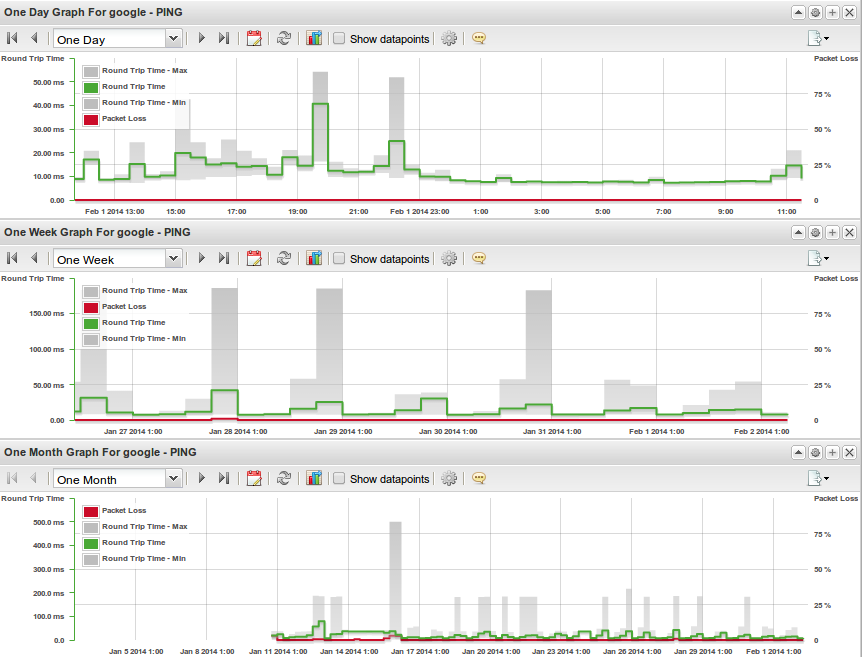
\includegraphics[width=1\textwidth]{img/pingiGoogle.png}
\end{figure}


Rysunki \ref{fig:google3001}, \ref{fig:google2801} oraz
\ref{fig:google2701} przedstawiają dokładniejsze dane z~przedziałów,
w~których notowano wzrosty czasu odpowiedzi. Analiza tych wykresów
pozwoliła na potwierdzenie tezy o~powtarzającej się tendencji. Łatwo
można zauważyć, że w~każdym z~pokazanych przedziałów notowany jest
stopniowy wzrost czasu odpowiedzi serwera od godziny 15. Godziny
wieczorne to na każdym z~wykresów zdecydowany wzrost czasu odpowiedzi,
a~także jego chwilowe skoki. Od około godziny 12 w~nocy pojawia się
spadek czasu odpowiedzi serwera, który utrzymuje się na niskim
poziomie aż do godziny 15. Uzyskane rezultaty są zgodne
z~oczekiwanymi. Okres, w~którym czas odpowiedzi serwera znacząco
wzrasta, przypada na tak zwane internetowe godziny szczytu, czyli
okres pomiędzy godziną 19 i 21. Zjawisko to zostało opisane
w~\cite{www:RushHours}.


\begin{figure}[H]
  \caption{Wykres wartości czasu podróży pakietu oraz stopnia
    utraconych pakietów dla {\em google.com} dnia 30.01.2014.}
  \label{fig:google3001}
  \centering
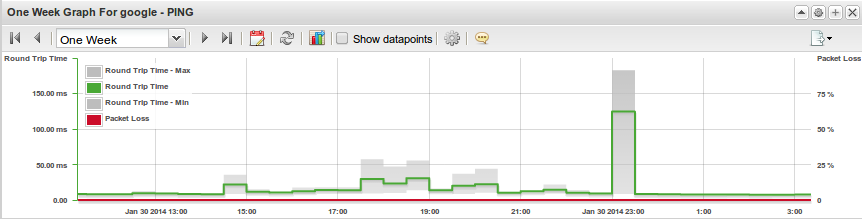
\includegraphics[width=1\textwidth]{img/google3001.png}
\end{figure}

\begin{figure}[H]
  \caption{Wykres wartości czasu podróży pakietu oraz stopnia
    utraconych pakietów dla {\em google.com} dnia 28.01.2014.}
  \label{fig:google2801}
  \centering
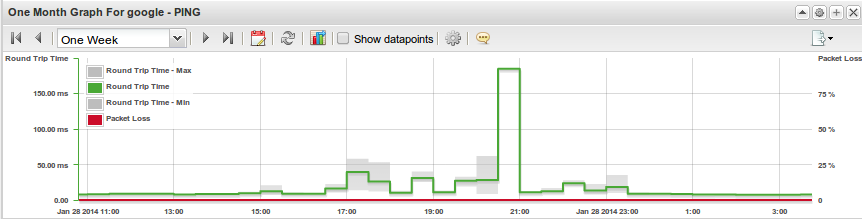
\includegraphics[width=1\textwidth]{img/google2801.png}
\end{figure}

\begin{figure}[H]
  \caption{Wykres wartości czasu podróży pakietu oraz stopnia
    utraconych pakietów dla {\em google.com} dnia 27.01.2014.}
  \label{fig:google2701}
  \centering
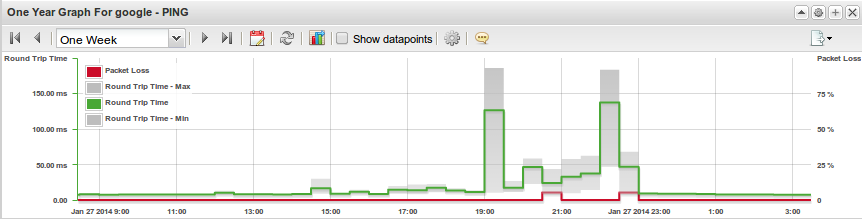
\includegraphics[width=1\textwidth]{img/google2701.png}
\end{figure}


\section[Klient mobilny][Rezultaty dla klientów mobilnych]{Rezultaty dla klientów mobilnych}

Monitorowanie klienta mobilnego odbyło się w~czasie jednego
tygodnia. Okres ten jest już znacznej długości, a~codzienne używanie
monitorowanych telefonów pozwoliło na wiarygodną symulację prawdziwych
warunków funkcjonowania systemu.

Przeprowadzone testy pozwoliły wykazać poprawność działania wszystkich
pożądanych mechanizmów. Pierwszym z~przetestowanych mechanizmów było
zapewnienie monitorowania stanu bieżącego usług i~parametrów urządzeń
mobilnych w~sposób analogiczny jak urządzeń statycznych. System
działał zgodnie z~oczekiwaniami, dzięki czemu wszystkie ostrzeżenia
były odpowiednio generowane. Przykładem takiego komunikatu jest
powiadomienie administratora o~stanie krytycznym baterii, które
zostało przedstawione na~rys.~\ref{fig:criticalBat}.

\begin{figure}[ht]
  \caption{Pulpit stanów poszczególnych usług i~parametrów klientów
    mobilnych.}
  \label{fig:criticalBat}
  \centering
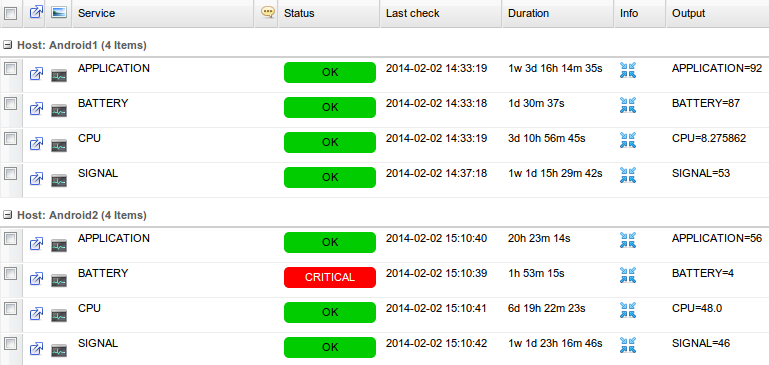
\includegraphics[width=1\textwidth]{img/criticalBat.png}
\end{figure}

Kolejną istotną funkcjonalnością, która była w~tym czasie testowana,
jest gromadzenie danych historycznych pochodzących od klienta
mobilnego. Mechanizm gromadzenia tych danych i~ich analizy działały
podczas testów bez zarzutu. Pozwoliło to na wykonanie wykresów
mierzonych wartości. Przykładowy wykres stanu baterii dla obu urządzeń
wygenerowany na podstawie danych zebranych w~czasie testów zawarto na
rysunku \ref{fig:baterie}.
 
\begin{figure}[ht]
  \caption{Wykres stanu baterii urządzeń mobilnych w okresie
    testowania systemu. Pierwszy wykres (u góry) pokazuje stan baterii
    urządzenia Android 1, drugi (na dole) --- urządzenia Android2.}
  \label{fig:baterie}
  \centering
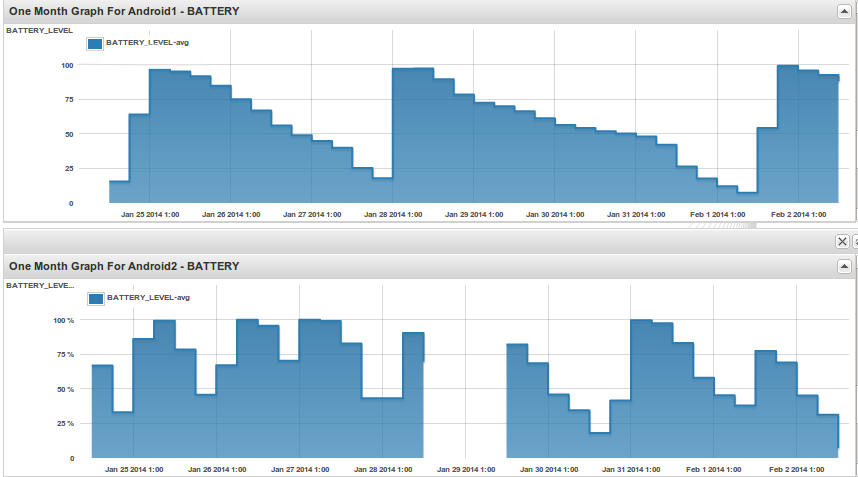
\includegraphics[width=1\textwidth]{img/battery.png}
\end{figure}

Widoczna na jednym z~wykresów przerwa wynika z~braku danych w~tym
okresie. Ze względu na równolegle powstawanie pracy inżynierskiej Pana
Marcina Kubika, który jest właścicielem tego urządzenia, konieczne
było wyłączenie go na jeden dzień. Na przedstawionych wykresach można
wyróżnić dwie fazy. Pierwsza z~nich to rozładowywanie baterii. Okres
ten można rozpoznać po zmniejszającym się pomiędzy kolejnymi pomiarami
stanem baterii. Okres ładowania widoczny jest na wykresie jako czas
gwałtownego wzrostu stanu baterii. Na podstawie wykresu można
oszacować, iż bateria urządzenia Android1 była ładowana 3 razy,
natomiast urządzenia Android2 co najmniej 6 razy. Wskazuje to na
znaczne zużycie baterii w~drugim urządzeniu lub jego bardzo intensywne
użytkowanie.

Ponadto na podstawie przedstawionego wykresu można wnioskować o~stylu
użytkowania obu telefonów. Urządzenie Android1 ładowane jest do bardzo
wysokiego poziomu baterii, a~następnie użytkownik oczekuje z jego
ładowaniem aż poziom baterii spadnie poniżej 20\%. Użytkownik
urządzenia Android2 natomiast bardzo często wykonuje ładowanie swojego
telefonu nawet przy stanie powyżej 50\%. W~zależności od typu baterii
znajdującej się w urządzeniu, takie działanie może skracać jej
żywotność. Dzięki długoterminowemu monitorowaniu tego typu zachowań
możliwe są badania wpływu profilu wykorzystania urządzenia na jego
żywotność i~awaryjność. Możliwość analizy sposobu użytkowania danego
urządzenia może być dla Administratora bardzo pomocne. Może to zostać
wykorzystane np. do lepszego zarządzania rozdziałem urządzeń mobilnych
w firmie. Ponadto jeśli monitorowane urządzenia mobilne posiadają
znaczną wartość, to śledzenie stylu ich użytkowania również jest
niezwykle istotne, aby zapewnić ich długą żywotność.

W~trakcie testów monitorowano również siłę sygnały Wi-Fi. Rezultaty
pomiarów przedstawiono na rysunku \ref{fig:signals}. Ponownie na
wykresie dla urządzenia drugiego widoczna jest przerwa wynikająca
z~chwilowego wyłączenia urządzenia. Na podstawie tych wykresów łatwo
można zauważyć, że urządzenie Android1 posiada znacznie częstszy
i~znacznie lepszy dostęp do sieci Wi-Fi niż urządzenie Android2. Można
wręcz zauważyć, iż urządzenie Android2 jest typowym klientem mobilnym,
który dostęp do sieci uzyskuje bardzo sporadycznie. Słaba siła sygnału
sieci Wi-Fi powoduje oczywiście zwiększone zużycie baterii, co jest
widoczne na wykresie z~rysunku~\ref{fig:baterie}.

\begin{figure}[ht]
  \caption{Wykres sygnału sieci Wi-Fi w okresie testowania
    systemu. Pierwszy wykres (u góry) pokazuje sygnał dla urządzenia
    Android1, drugi (na dole) --- urządzenia Android2.}
  \label{fig:signals}
  \centering
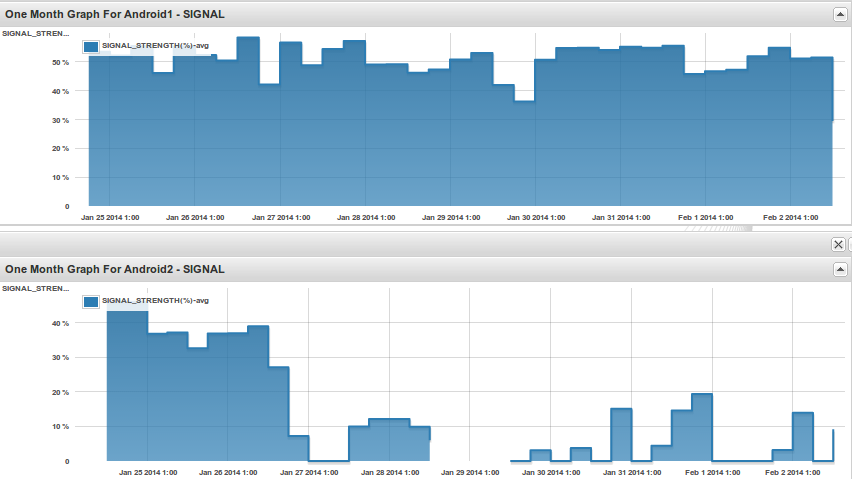
\includegraphics[width=1\textwidth]{img/wifi.png}
\end{figure}

W~zastosowaniu produkcyjnym analiza takich danych jak dostępność sieci
Wi-Fi w~miejscu codziennego użytku urządzenia mobilnego jest niezwykle
istotna. Firmy wydają bardzo duże pieniądze na zakup pakietów danych
u~operatorów sieci komórkowych w~celu zapewnienia swoim pracownikom
łączności z~Internetem. Na podstawie analizy siły sygnału sieci dla
każdego klienta można w~dużo lepszy sposób zarządzać limitami danych
otrzymanymi od operatora. Jeśli część klientów mobilnych przebywa
przez większość czasu w~zasięgu sieci Wi-Fi, to być może należy
ograniczyć przyznane dla nich limity na rzecz zwiększenia
przepustowości sieci bezprzewodowej. Ponadto dane o~sile sygnałów
pochodzące z~wielu urządzeń pozwalają na badanie wpływu rozmieszczenia
punktów dostępowych na zasięg sieci w~siedzibie firmy.
